\chapter{Adding Memory to the Agents}
\section{Overview}
Until now, we have assumed that all of the problems are fully observable, which means that they follow an MDP. The assumption behind this is that using the information given by the observation of the environment should be sufficient to fully understand its state. Thus:

\begin{equation}
    o_{t} = s_{t}
\end{equation}

But this is not always true and D-COACH is not suited to perform well in POMDPs. There are different reasons of why a problem is partially observed. In this work we focus on those cases where the observations represent instant information sensed from the environment but the state is described by time-dependent phenomena. For instance, if we want to estimate the velocity of a flying drone using information obtained from an RGB camera, it is necessary to combine data from different time steps in order to achieve this. 

In this chapter we aim to use a function approximation model that adds memory to the agents and to propose a variation of D-COACH which is capable of training this model. The idea is to validate this approach through simulations, establishing a baseline for further research in memory-based deep interactive learning.

\section{Method}
There are two well-known approaches for adding memory to agents in sequential decision-making problems when using DNNs as function approximator:

\begin{enumerate}
    \item \textbf{Observation stacking: \textbf{CITE}} This approach consists of stacking a fixed number of past observations to the current one and using this modified observation as the input of the policy. 
    \item \textbf{Recurrent models: \textbf{CITE}} This approach consists of using policies based on RNNs. Given that these models have an internal state, they can store information from the past (i.e. they have memory) and use it in posterior inferences. 
\end{enumerate}

One of the main issues of observation stacking is that the memory of this model is determined by the number of stacked observations. In high-dimensional state problems, the size of the input can increase considerably as the number of stacked observations increment, producing an overhead that makes this approach impractical. 

On the other hand, in RNNs the overhead is determined by the size of its hidden layers and the size of the sequences used when updating the weights of the model. As a consequence, the most important overhead of RNNs occurs when training. Several DRL approaches have used this approach without reporting large overheads \textbf{CITE}.

Given the more practical usage of recurrent models, in this work we use RNNs policies to test the viability of D-COACH for solving problems in a POMDP setting. 

\subsection{Learning to Remember}
Even though RNNs are networks with the capability of storing/summarizing information from past observations, they have to learn to do this. Commonly, in DRL approaches, this is not treated as a separated issue and the error of the cost function is propagated through the RNN as it would be done with other architectures. 

This may give the intuition that using D-COACH with RNNs would only require to change the FNN or CNN models with an RNN. Nevertheless, preliminary tests showed that shaping RNN-based policies with D-COACH made the agents to rapidly overfit to the first set of corrections, loosing the capability of learning interesting behaviors and, as a consequence, solving tasks. 

To overcome this shortcoming, we propose to use RNN layers to learn the dynamics of the environment, similarly as in \cite{Ha2018}. This approach take ideas from model-based RL in the sense that a model of the environment is learned. The difference is that in this case the model is learned such that the RNN layers learn to embed the past in its hidden state, but no planning or control techniques are used. In a nutshell, we want to learn the function $M(s_{t}, a_{t})$ as stated in Equation \ref{eq:model}:

\begin{equation}
    M(s_{t},a_{t}) = s_{t+1}
\end{equation}


\subsection{Low-dimensional State with Memory}
As it has been done previously in this work, we first study the low-dimensional state case. The objective is to learn the dynamics of the environment online i.e. as the policy is shaped interactively. 

If we look back to Chapter 2, the problem was similar. In that case the objective was to learn a low-dimensional embedding of a high-dimensional input online. The strategy was to share the encoder layers of an autoencoder between the policy and the autoencoder and update them using both the cost of the policy and the one of the autoencoder. In this case, we could see the hidden state of the recurrent layers as an embedding of past observations and share this layers between the policy and the model, updating them using both costs. The problem with this approach in this case is the one observed in the preliminary tests, the cost of the policy does not work well when updating the weights of recurrent layers.  

So, alternatively, the taken approach was to update the recurrent layers online only using the cost of the model and using the output of these layers as the input of FNN layers that are shaped using the policy cost. The model is updated with data collected while the agent is learning the policy. The general structure of this approach is shown in Figure \ref{fig:rnn_ld}.

\begin{figure}[h]
    \centering
    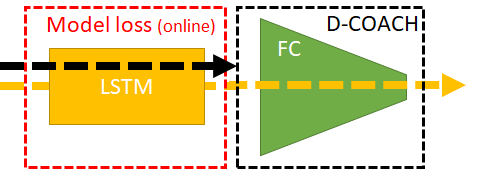
\includegraphics[width=0.5\linewidth]{imagenes/cap4/RNN_LD.png}
    \caption{Low-dimensional architecture for POMDP problems.}
    \label{fig:rnn_ld}
\end{figure}

The yellow arrow shows the flow of data when evaluating the network. The black arrow shows the flow of data when using the replay buffer to update the FNN layers. To train the FNN layers from the replay buffer a mini-batch is sampled, then is evaluated through the recurrent layers and finally is used as input of these layers (instead of directly storing the hidden state of the recurrent layers in the replay buffer).

\subsection{High-dimensional State with Memory}
In the high-dimensional case the agent needs to learn two embeddings: the one of the autoencoder, and the one of the model. In the preliminary tests, we found that the most effective way of doing this under the setting of D-COACH is to treat the autoencoder and the recurrent layers as one architecture, which represents the model. A model with the capability of learning from high-dimensional states, as it can be seen in Figure \ref{fig:rnn_hd}. 

\begin{figure}[h]
    \centering
    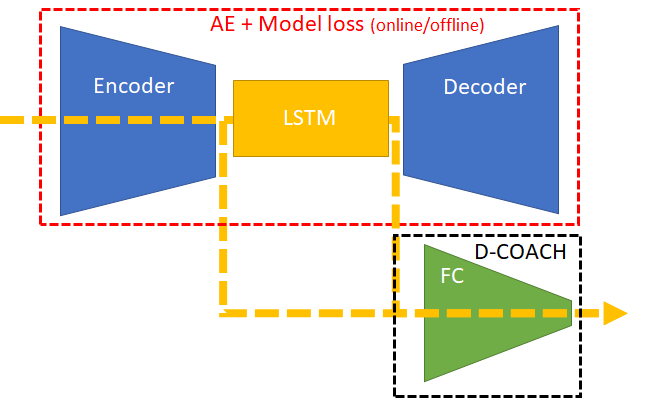
\includegraphics[width=0.6\linewidth]{imagenes/cap4/RNN_HD.png}
    \caption{High-dimensional architecture for POMDP problems.}
    \label{fig:rnn_hd}
\end{figure}

Instead of using a cost for the model and one for the autoencoder, we use the autoencoding cost but for reconstructing $s_{t+1}$. So, Equation \ref{eq:ae} instead of being $L(x_{t},\widetilde x_{t})$ it would be  $L(x_{t},\widetilde x_{t+1})$. The idea behind is to give memory to the autoencoder, so that can reconstruct future observations. By doing this, the output of the recurrent layers embed both the high-dimensional input and past observations.

\subsection{The Algorithm}

\section{Experiments and Results}
Simulated teachers were used in three different problems for validating this version of D-COACH. The main idea behind these experiments is to compare D-COACH with and without memory in partially observed problems. For high-dimensional states, the online state learning version of D-COACH without memory is used, given that is faster to use and its performance is similar to the offline state learning version. 

\begin{enumerate}
    \item \textbf{Partially Observed Cart-Pole:} A partially observed low-dimensional state scenario. This is the same environment used in Chapter 1 with a modification in the observation space of the agent. In the standard fully-observable cart-pole the state has four dimensions, which consist on the position $x$ and velocity $\dot x$ of the cart and the angle $\theta$ and angular velocity $\dot \theta$ of the pole, such that $s=[x, \dot x, \theta, \dot \theta]$. In this case, we take out the derivatives present in the state, such that $s=[x, \theta]$.
    \item \textbf{Partially Observed Cart-Pole from Pixels:} Again, the cart-pole environment is modified to use as input raw pixels (high-dimensional state). 
    \item \textbf{Partially Observed Car Racing:} A partially observed high-dimensional state scenario. The Car Racing environment previously used is modified such that the indicators in the bottom of the image are erased. 
    
\end{enumerate}

\subsection{Validation Low-Dimensional State}

D-COACH with model is tested in the partially observed cart-pole because is a way to validate if the proposed methodology works in a simple setting. Figure \ref{fig:ld_cartpole_model} shows the learning curves of D-COACH with and without model. 

\begin{figure}[h]
    \centering
    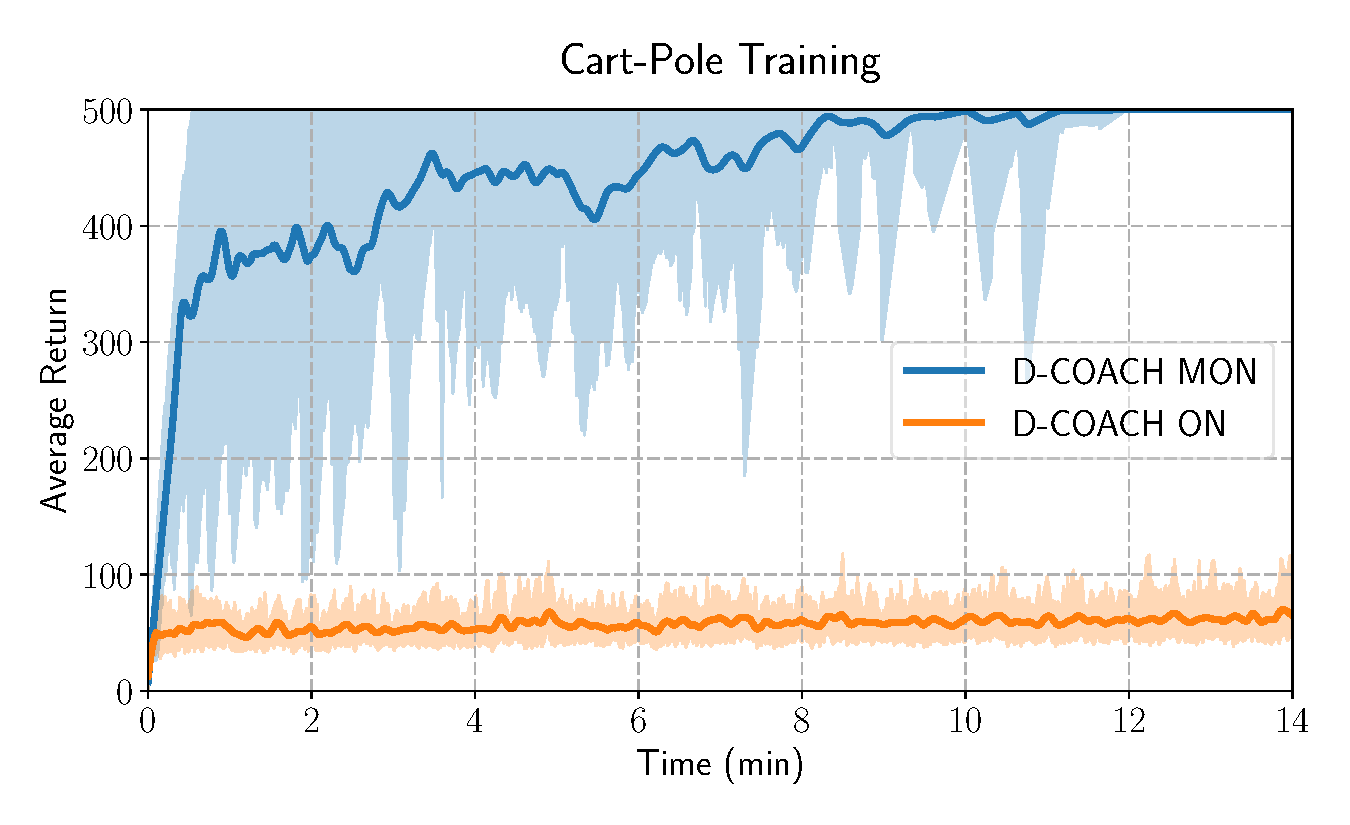
\includegraphics[width=0.9\linewidth]{imagenes/cap3/cartpole_LD_model.pdf}
    \caption{Evolution of the error while learning the reacher task. }
    \label{fig:ld_cartpole_model}
\end{figure}

D-COACH without model is not able to learn a well performing policy in this case. This was something to expect given that the velocities of both the cart and the pole are essential for making good decisions in a problem of this characteristics. Figure \ref{fig:cp_ex} shows and example of two scenarios in where at time step 2 the observation would be the same in the partially observed cart-pole (if we only focus on the angle of the pole). In this example the angular velocity of the pole changes direction between scenarios, but an agent without memory is not able to tell the difference. As a consequence, in $t=2$, it would make the same decision in two opposite scenarios.

\begin{figure}[h]
    \centering
    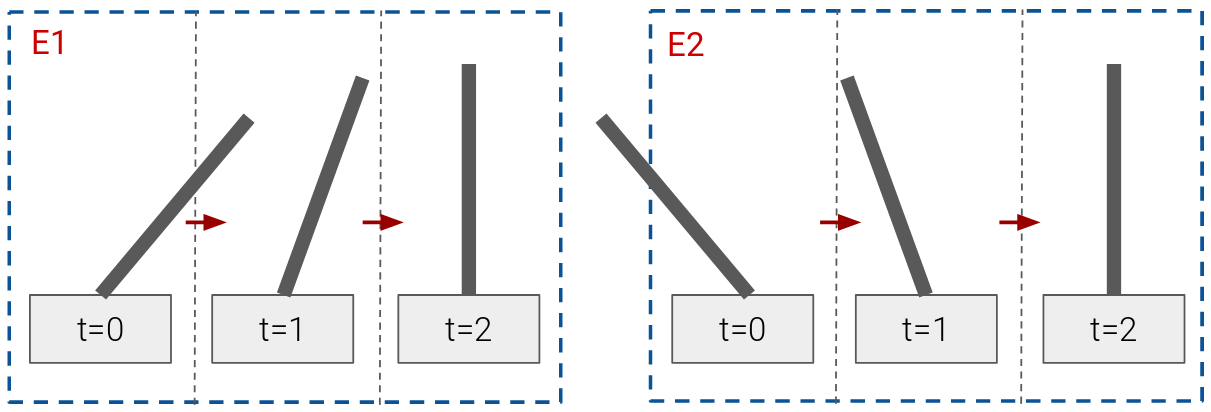
\includegraphics[width=0.9\linewidth]{imagenes/cap4/cartpole_ex.png}
    \caption{Evolution of the error while learning the reacher task. }
    \label{fig:cp_ex}
\end{figure}

In contrast, if the agent makes decisions based on previous observations it can understand that these two scenarios are different, and as a consequence, make better decisions. This is shown in the blue curve of Figure \ref{fig:cp_ex}, where the agent is able to learn a well performing policy in about 14 minutes. 

Finally, in  Figure \ref{fig:cp_ex} both curves, at the end of the first minute, achieve a peak in performance, which is followed by a deterioration. In the case of the policy with model the agent is able to recover and learn a good behavior eventually, while the policy with no memory is not. This peak occurs because, at the beginning of the learning process, the percentage of time steps in which the simulated teacher gives feedback is high ($\sim 50-60 \%$). These corrections modify the policy instantly, so the agent is "guided" by the teacher. As the percentage of feedback signals decreases, also does this "guidance" effect. If the agent is able to learn a well performing policy, then it should recover (like the blue curve); otherwise, it should not. Depending on the parameters of the function that defines the probability of the simulated teacher of making a correction this effect may appear, as in this case.

\subsection{Validation High-Dimensional State}
In this section we validate D-COACH with memory in two different problems. Cart-pole is a problem that was not originally designed to be solved using as input raw pixels of an image, so we do not expect to obtain a perfect performance in this case. The main goal of testing D-COACH with this problem is to observe if the proposed model (autoencoder + LSTM) is able to embed both the past and high-dimensional inputs adequately. As it was seen in Figure \ref{fig:cp_ex}, it should not be possible (or much more difficult) to solve the cart-pole problem mwith partial observability.

\begin{figure}[h]
    \centering
    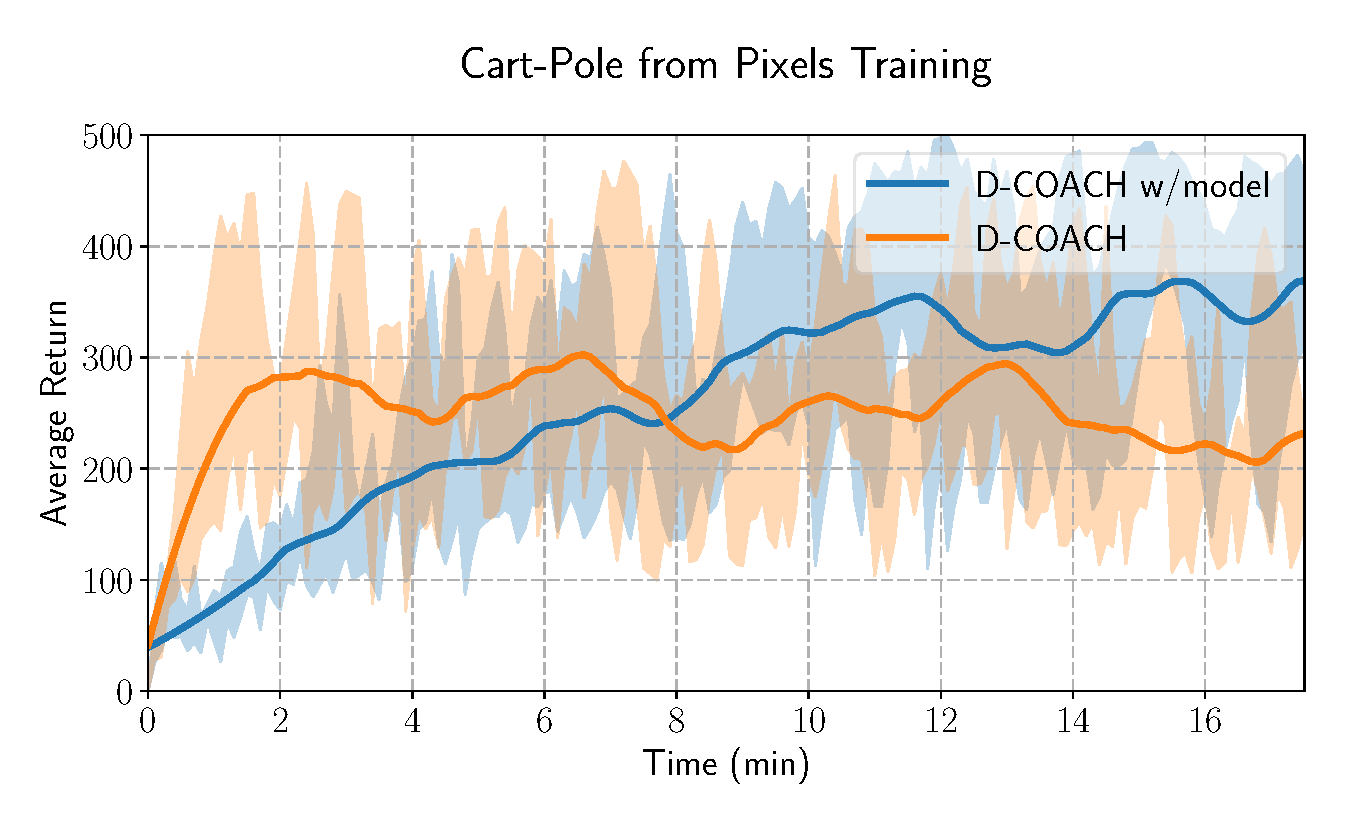
\includegraphics[width=0.9\linewidth]{imagenes/cap3/cartpole_HD_model.pdf}
    \caption{Evolution of the error while learning the reacher task. }
    \label{fig:cp_hd}
\end{figure}

Figure \ref{fig:cp_hd} shows a much more slower learning speed if we compare these agents with the ones of Figure \ref{fig:cp_ex}. This is something to expect given that now the agents are also learning to extract features from the image. Also, model-free D-COACH shows a faster learning speed at the beginning, but after 8 minutes of learning it is outperformed by model-based D-COACH. This shows that D-COACH takes longer to learn a time/space embedding, than just a space embedding. But, in POMDPs, eventually, model-based D-COACH should outperform its model-free version.

Finally, model-based D-COACH was validated in the partially observed Car Racing problem. Figure \ref{fig:po_cr} shows that model-free D-COACH is able to learn a well-performing policy even though the state is partially observed. Nevertheless, model-based D-COACH shows that it is possible to obtain an even better performance if memory is added to the policy. The difference between both curves shows that model-based D-COACH is a more robust and powerful approach in problems where model-free D-COACH could appear to be sufficient.

\begin{figure}[h]
    \centering
    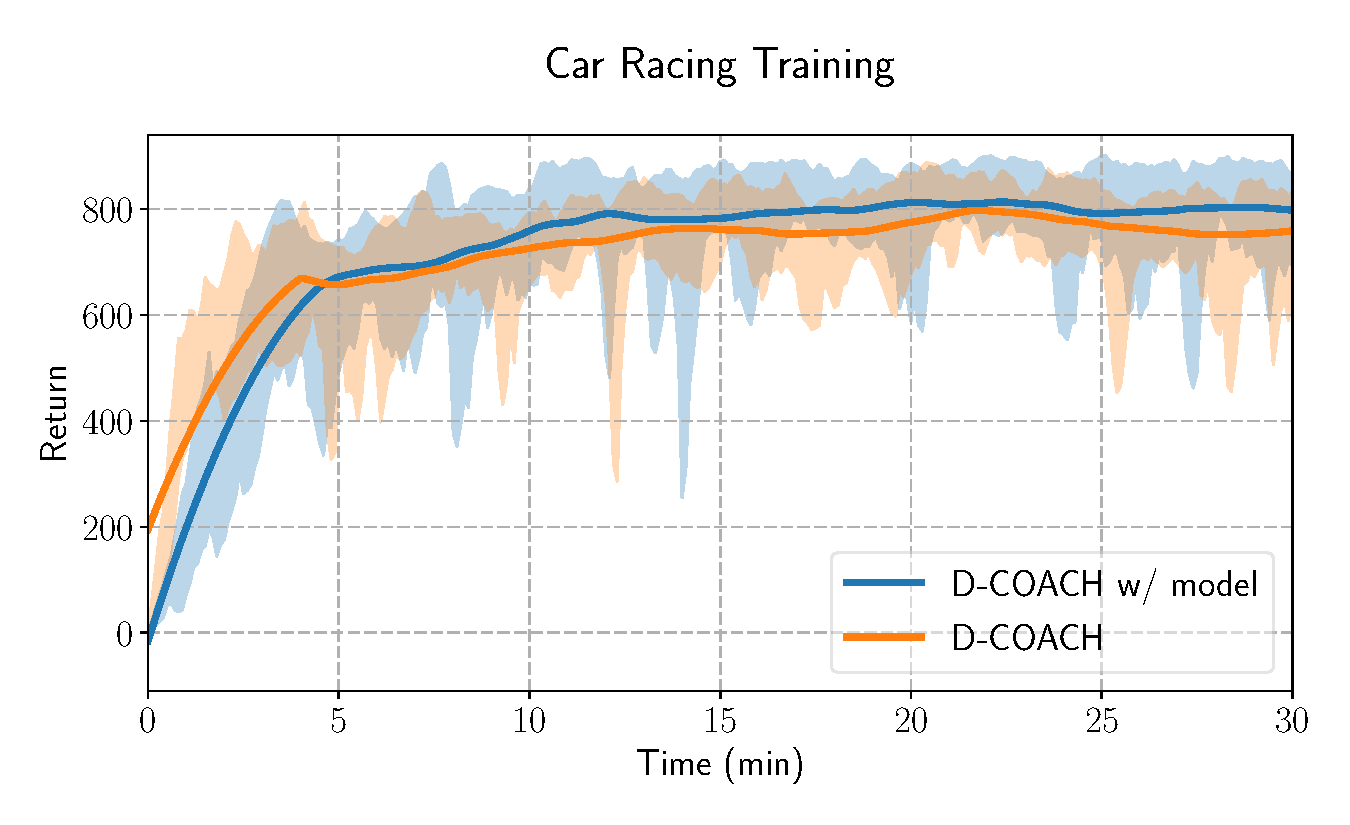
\includegraphics[width=0.9\linewidth]{imagenes/cap3/car_racing_lstm.pdf}
    \caption{Evolution of the error while learning the reacher task. }
    \label{fig:po_cr}
\end{figure}